%%%%%%%%%%%%%%%%%%%%%%%%%%%%%%%%%%%%%%%%%%%%%%%
\chapter{Network Coding} \label{chap:network_coding}
%%%%%%%%%%%%%%%%%%%%%%%%%%%%%%%%%%%%%%%%%%%%%%%

\section{What is Network Coding? \label{sec:What-is-NC}}

We first explain the term of network, then we futher introduce Network
Coding. Our considered communication network is a directed graph\footnote{Network coding over undirected networks was introduced in \cite{Li:2004}.}
allowing multiple links from one node to another. Each \textit{link}
in a network has \textit{unit capacity}, i.e. it carries a packet
which is either a symbol from $\ensuremath{\mathbb{F}}_{q_{\mathrm{s}}}$,
or a vector of length $t$ over $\ensuremath{\mathbb{F}}_{q}$. Note
that the assumption of unit capacity does not restrict our considered
networks in Section \ref{sec:Description_GCN}, since links of larger
capacity can be represented by multiple parallel links $\ell$ of
a data unit. In Figure \ref{fig:incoming_links}(a), a node of a network
is represented with its \textit{incoming} and \textit{outgoing }links
. A node without any incoming link is a \textit{source} node of the
network. Packets are transmitted from the source to a set of destination
nodes, i.e. \textit{receivers}, over error-free links, which is still
applicable to present-day wireline networks\footnote{Wireless network coding was introduced in \cite{Katti:2008}.}.

\begin{figure}[H]
\caption{Incoming links and outgoing links of a node in network coding \label{fig:incoming_links}}

\centering{}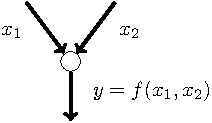
\includegraphics[height=0.1\paperwidth]{E:/Documents/TUM/THESIS/thesisCOD_Ha/figures/incoming_edges}
\end{figure}

In simple routing, information is transmitted from the source to receivers
through a chain of \textit{intermediate nodes} by a method known as
store-and-forward \cite{Yeung:2006}. In this method, the information
transmission can be represented as \textit{packet transmission}s on
links and the packets received from an incoming link of an intermediate
node, i.e. \textit{incoming packets}, can only be forwarded to a next
node via an outgoing link as its \textit{outgoing packets}. \textit{Network
coding} was though first introduced in Ahlswede et al.'s seminal paper
\cite{Ahlswede:2000} as ``coding at a node in a network'', where
coding means an arbitrary combination of received packets on a node's
incoming links for an outgoing packet. It means that each intermediate
node in the network (not only at the source) is allowed to forward
a \textit{function} of their incoming packets, e.g. $y_{1}=f_{1}(o_{1},o_{2})$
in Figure \ref{fig:incoming_links}. These functions are not required
to be injective functions, i.e. some outgoing packets can be duplicated
from a map of same incoming packets, which motivates our study in
Section \ref{sec:Network_e1l1h3rs4}. A \textit{network code} is a
set of these functions of the packets on the links of the network
\cite{Wachter-Zeh:2018}. A network code is called a \textit{solution}
for the network or the network is \textit{solvable}, if there exists
an assignment of all the functions on all the links of the network
such that each receiver can recover its requested packets from its
incoming packets. If these functions are linear, we obtain a \textit{linear
network coding solution}, and we do not consider \textit{nonlinear
solution} throughout this thesis. Each function on a link consists
of \textit{coding coefficients} for each incoming packet. The coding
coefficients form a coefficient vector whose length is equal to the
number of each node's incoming links, and this coefficient vector
is called the \textit{local coding vector}, which is distinguished
with \textit{global coding vector} defined in Section \ref{subsec:Matrix-channel}.
If the coding coefficients and the packets are scalars, a solution
of linear network coding is called \textit{scalar solution}. Based
on these coding coefficients, Kötter and M\'edard provided in \cite{Koetter:2003}
an algebraic formulation for the linear network coding problem and
its scalar solvability.

\section{Advantages of Network Coding \label{sec:Advantages-of-NC}}

\paragraph{Throughput gain and reduced complexity}

Network coding gives a potential gain in throughput by communicating
more information with fewer packet transmissions compared to the routing
method. The butterfly network in \cite{Ahlswede:2000} as a multicast
in a wireline network is a standard example for an increase of throughput.

\begin{figure}[H]
\caption{The butterfly network \label{fig:The-butterfly-network}}

\centering{}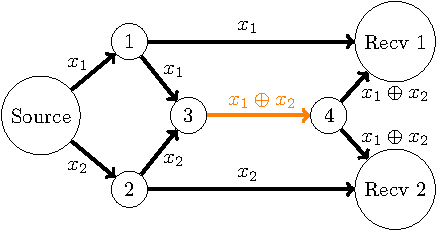
\includegraphics[width=0.5\paperwidth]{E:/Documents/TUM/THESIS/thesisCOD_Ha/figures/ahlswede_butterfly_network}
\end{figure}

In Figure \ref{fig:The-butterfly-network}, we denoted a receiver
by ``Recv'', which is used for all of figures in this study. With
the help of network coding, both Recv 1 and Recv 2 can recover $x_{1}$
and $x_{2}$ by a bitwise XOR in Figure \ref{fig:The-butterfly-network}(c).
Without network coding, an additional transmission between Node 3
and 4 must be supplemented to communicate the contents of 2 packets
$x_{1}$ and $x_{2}$ from the source to Recv 1 and Recv 2, i.e. we
must communicate $x_{1}$ or $x_{2}$ separately on this link twice
under routing in Figure \ref{fig:The-butterfly-network}(a) and (b). 

\paragraph{Robustness and security}

\textit{Packet loss} is a particular issue in wireless packet networks
due to several reasons, e.g. buffer overflow or communication failures
\cite{Ho:2008}. Sharing a common concept with Erasure Coding (EC)
by exploiting a degree of redundancy to packets on any vertices in
the network, the receivers are able to successfully recover the original
packets from a large number of packet losses, e.g. $101\circledast10\circledast1$.
The only difference is that packets are only encoded by the source
in EC \cite{Fujimura:2008}. This problem is dealed by acknowledgement
messages in the mechanism of transmission control protocol (TCP) \cite{Ho:2008}.
Network coding offers both benefits and drawbacks regarding to security.
For example, node 4 is operated by an eavesdropper and it obtains
only the packet $x_{1}\oplus x_{2}$, so it cannot obtain either $x_{1}$
or $x_{2}$ and the communication is secure. Alternatively, if the
eavesdropper controls node 3, it can anonymously send a fake packet
masquerading as $x_{1}\oplus x_{2}$, which is difficult to detect
in network coding \cite{Ho:2008}.

\paragraph{From scalar network coding to vector network coding}

Ebrahimi and Fragouli \cite{Ebrahimi:2011} have extended the algebraic
approach in \cite{Koetter:2003} to \textit{vector network coding}.
Here, all packets are vectors of length $t$, and the coding coefficients
are $\left[t\times t\right]$ matrices. The network code is therefore
a set of functions consisting of $\left[t\times t\right]$ coding
matrices, and is called \textit{vector solution} if all receivers
can recover their requested information for such coding marices. The
motivation of vector netwok coding is that there exists networks do
not have scalar solutions, but are solvable by vector routing, e.g
\cite{Medard:2003}. Although it was shown that not every solvable
network has a vector solution in \cite[Lemma II.2]{Dougherty:2005},
Das and Rai proved in \cite{Das:2016} that there exists a network
with a vector solution of dimension $m$ but with no vector solution
over any finite field whose the dimension is less than $m$. When
we refer the \textit{alphabet size} of a network coding solution,
we mean the field size $q_{\mathrm{s}}$ or $q_{v}$ of the finite
field $\ensuremath{\mathbb{F}}_{q_{\mathrm{s}}}$ or $\ensuremath{\mathbb{F}}_{q_{v}}$
respectively for such a scalar solution or a vector solution. The
alphabet size is an important parameter determining the amount of
computation performed at each network vertice \cite{Wachter-Zeh:2018}.
The problem of finding the minimum required alphabet size of a (linear
or nonlinear) scalar network code for a certain multicast network
is NP-complete \cite{Langberg:2009,Lehman:2004,Gone:2018}. This thesis
focuses on determining the sovability of networks to measure the gap,
and our considered networks in Section \ref{sec:Description_GCN}
consist only error-free links, we therefore do not consider error
correction here. Furthermore, we consider the solvability of networks
by proving an existence of an assignment for all functions such that
all receiver can recover its requested information, so the functions
or coding coefficients are clearly chosen instead of being arbitrary
or random as the ones used in \cite{Ho:2003,Ahlswede:2000}. We later
distinguish scalar and vector network coding more specifically in
Section \ref{subsec:Matrix-channel} and \ref{sec:Network-Coding-for-GCN}.

\section{Network as a matrix channel \label{subsec:Matrix-channel}}

To formulate a network coding problem, the source has a set of disjoint
messages referred to packets on links which are either symbols from
$\ensuremath{\mathbb{F}}_{q_{\mathrm{s}}}$ (scalar coding) or vectors
of length $t$ over $\ensuremath{\mathbb{F}}_{q}$ (vector coding)
as mentioned in Section \ref{sec:What-is-NC}. Each receiver $R_{j},j\in\left\{ 1,\ldots,N\right\} $
requests a subset of same $h$ messages from the source. Through all
the functions on the links from the source to each receiver, the receiver
obtains several linear combinations of the $h$ messages to form a
linear system of equations for its requested messages. The coefficients
of a linear combination is called \textit{global coding vector} \cite{Sanders:2003}.
The linear equation system that any receiver $R_{j}$ has to solve
is as following:

\begin{equation}
\begin{array}{c|c}
Scalar & Vector\\
\underset{\ensuremath{\mathbb{F}}_{q_{\mathrm{s}}}^{s}}{\underbrace{\left[\begin{array}{c}
y_{j_{1}}\\
\vdots\\
y_{j_{s}}
\end{array}\right]}}=\underset{\ensuremath{\mathbb{F}}_{q_{\mathrm{s}}}^{s\times h}}{\underbrace{\boldsymbol{A}_{j}}}\cdot\underset{\ensuremath{\mathbb{F}}_{q_{s}}^{h}}{\underbrace{\left[\begin{array}{c}
x_{1}\\
\vdots\\
x_{h}
\end{array}\right]}} & \underset{\ensuremath{\mathbb{F}}_{q}^{st}}{\underbrace{\left[\begin{array}{c}
\boldsymbol{y}_{j_{1}}\\
\vdots\\
\boldsymbol{y}_{j_{s}}
\end{array}\right]}}=\underset{\ensuremath{\mathbb{F}}_{q}^{st\times th}}{\underbrace{\boldsymbol{A}_{j}}}\cdot\underset{\ensuremath{\mathbb{F}}_{q}^{th}}{\underbrace{\left[\begin{array}{c}
\boldsymbol{x}_{1}\\
\vdots\\
\boldsymbol{x}_{h}
\end{array}\right]}}
\end{array}\label{eq:linear_system}
\end{equation}

The transfer matrix $\boldsymbol{A}_{j}$ contains the links' global
coding vectors, which are combined by the coefficients of linear combinations
on $\alpha l$ links from $\alpha$ nodes and $\epsilon$ direct-links
to the corresponding receiver $R_{j}$:

\[
\begin{array}{c|c}
Scalar & Vector\\
\boldsymbol{A}_{j}=\left[\begin{array}{c}
\boldsymbol{a}_{j_{1}}\\
\vdots\\
\boldsymbol{a}_{j_{\alpha\ell}}\\
\vdots\\
\boldsymbol{a}_{j_{\alpha\ell+\epsilon}}
\end{array}\right] & \boldsymbol{A}_{j}=\left[\begin{array}{c}
\boldsymbol{A}_{j_{1}}\\
\vdots\\
\boldsymbol{A}_{j_{\alpha l}}\\
\vdots\\
\boldsymbol{A}_{j_{\alpha l+\epsilon}}
\end{array}\right]
\end{array}
\]

In general, the network is represented as a matrix channel for both
scalar and vector coding: $\boldsymbol{Y}_{j}=\boldsymbol{A}_{j}\cdot\boldsymbol{X}$.
In our study, the network structure is known, i.e. we reconstruct
$\boldsymbol{X}$ with knowing $\boldsymbol{A}_{j}$, so our network
is coherent. A network is \textit{sovable} or a network code is a
\textit{solution}, if each receiver can reconstruct its requested
messages or solve the system with a unique solution for scalars $x_{1},\ldots,x_{h}$,
or vectors $\boldsymbol{x}_{1},\ldots,\boldsymbol{x}_{h}$. In network
coding problems, we want to find global coding vectors such that the
matrix $\boldsymbol{A}_{j}$ has full-rank for every $j=1,\ldots,N$,
and such that $q_{\mathrm{s}}$ or $q^{t}$ is minimized as mentioned
in Section \ref{sec:Advantages-of-NC}. In Example \ref{ex:scalar_vector_mapping},
we provide a vector solution of field size $q$ and dimension $t$,
which has the same alphabet size as a scalar solution of field size
$q^{t}$.

To summarize the notations of both scalar and vector coding, we represent
them as in Table~\ref{tab:notations}:

\begin{table}[H]
\caption{Notations of network coding}

\label{tab:notations} 
\centering{}%
\begin{tabular}{|>{\centering}p{0.2\paperwidth}|c|c|}
\hline 
 & Scalar Coding & Vector coding\tabularnewline
\hline 
\hline 
Source Messages/Packets & $\begin{array}{c}
x_{1},\ldots,x_{h}\in\ensuremath{\mathbb{F}}_{q_{\mathrm{s}}}\\
\boldsymbol{x}\in\ensuremath{\mathbb{F}}_{q_{\mathrm{s}}}^{h}
\end{array}$ & $\begin{array}{c}
\boldsymbol{x}_{1},\ldots,\boldsymbol{x}_{h}\in\ensuremath{\mathbb{F}}_{q}^{t}\\
\boldsymbol{x}\in\ensuremath{\mathbb{F}}_{q}^{th}
\end{array}$\tabularnewline
\hline 
Global Coding Vectors Of Receiver $R_{j}$ & $\boldsymbol{a}_{j_{1}},\ldots,\boldsymbol{a}_{j_{s}}\in\ensuremath{\mathbb{F}}_{q_{\mathrm{s}}}^{h}$ & $\boldsymbol{A}_{j_{1}},\ldots,\boldsymbol{A}_{j_{s}}\in\ensuremath{\mathbb{F}}_{q}^{t\times th}$\tabularnewline
\hline 
Transfer Matrix Of Receiver $R_{j}$ & $\boldsymbol{A}_{j}\in\ensuremath{\mathbb{F}}_{q_{\mathrm{s}}}^{s\times h}$ & $\boldsymbol{A}_{j}\in\ensuremath{\mathbb{F}}_{q}^{st\times th}$\tabularnewline
\hline 
Packets On Receiver $R_{j}$ & $\begin{array}{c}
y_{j_{1}},\ldots,y_{j_{s}}\in\ensuremath{\mathbb{F}}_{q_{\mathrm{s}}}\\
\boldsymbol{y}\in\ensuremath{\mathbb{F}}_{q_{\mathrm{s}}}^{s}
\end{array}$ & $\begin{array}{c}
\boldsymbol{y}_{j_{1}},\ldots,\boldsymbol{y}_{j_{s}}\in\ensuremath{\mathbb{F}}_{q}^{t}\\
\boldsymbol{Y}_{j}\in\ensuremath{\mathbb{F}}_{q}^{st}
\end{array}$\tabularnewline
\hline 
Number of nodes & $r_{scalar}$ & $r_{vector}$\tabularnewline
\hline 
\end{tabular}
\end{table}

\begin{rem}
By using the vector coding, the upper bound number of solutions increases
from $q^{tkh}$ to $q^{t^{2}kh}$. Therefore, vector network coding
offers more freedom in choosing the coding coefficients than does
scalar linear coding for equivalent alphabet sizes, and a smaller
alphabet size might be achievable \cite{Ebrahimi:2011}. By this advantage,
we can have higher number of receivers, i.e. higher number of nodes,
in vector network coding.
\end{rem}

\section{Network Model}

\subsection{Multicast Networks as Generalized Combination Networks}

A class of networks which is mainly studied is the class of multicast
networks. It can be one-to-many or many-to-many distribution \cite{Harte:2008}.
In this study, we target one-to-many multicast network with the distribution
of a data packet to a group of users \cite{Zhang:2012}. An interesting
network structure often used for multicast networks in network coding
is called Combination Network (CN) and denoted by $\mathcal{N}_{h,r,s}$.
Many examples in previous studies demonstrating the advantage of network
coding have used structures identical or similar to that of CN. We
mention a few examples to emphasize CN's importance in the study of
network coding. In Figure \ref{fig:butterfly_nw_cn}, the butterfly
network that is often used as a first example to motivate network
coding, e.g. \cite[Fig. 7]{Ahlswede:2000} and \cite[Fig. 1]{Sanders:2003},
is isomorphic to $\mathcal{N}_{h,r=3,s=2}$, if we consider it as
an undirected network \cite{Maheshwar:2012}. The $\mathcal{N}_{h,r=3,s=2}$
itself was also used in the first study of network coding \cite{Ahlswede:2000}.
Other CNs, i.e. $\mathcal{N}_{h,r=4,s=2}$ and $\mathcal{N}_{h,r=6,s=3}$,
were also used as examples to demonstrate the advantage of network
coding in \cite[Fig. 2]{Sanders:2003} and \cite[Fig. 2]{Jaggi:2005}
respectively. The general structure of CN was also introduced and
discussed in \cite[Sec. 4.3]{Fragouli:2006}, \cite[Sec. 4.1]{Yeung:2006},
\cite{Ngai:2004,Xiao:2007}.
\begin{figure}[H]
\caption{The butterfly network is represented as a combination network \label{fig:butterfly_nw_cn}}

\centering{}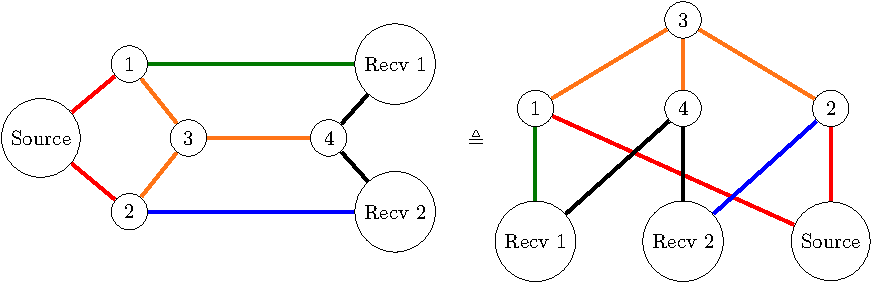
\includegraphics[width=0.5\paperwidth]{E:/Documents/TUM/THESIS/thesisCOD_Ha/figures/ahlswede_butterfly_network_CN}
\end{figure}

A generalization of a CN \cite{Riis:2006} is called generalized combination
network (GCN). GCN defined in \cite{Etzion:2016,Wachter-Zeh:2018}
was used to prove that vector network coding outperforms scalar linear
network coding , in multicast networks, with respect to the \textit{alphabet
size}, using rank-metric codes and Grassmannian codes. A comparison
between the required alphabet size for a scalar linear solution, a
vector solution, and a scalar nonlinear solution, of the same multicast
network is an important problem. Etzion and Wachter-Zeh introduced
a \textit{gap} in \cite{Etzion:2016} as the difference between the
smallest alphabet size for which a scalar linear solution exists and
the smallest alphabet size for which they can construct a vector solution.
They have found bounds on the gap for several network families of
GCN in \cite{Etzion:2016,Wachter-Zeh:2018}, but no gap for the GCN
networks with 3 messages has been found, i.e. $(1,1)-\mathcal{N}_{3,r,4}$,
where we denote GCN by $(\epsilon,l)-\mathcal{N}_{h,r,s}$. Therefore,
a combinatorial approach is first introduced in this thesis to prove
an existence of a vector solution outperforming the optimal scalar
linear solution with $q^{t^{2}/4+\mathcal{O}(t)}$. We then further
extend the approach for a family of GCN called One-Direct Link Combination
Network, i.e. $(1,1)-\mathcal{N}_{h,r,s}$. More formal definitions
of the gap and GCN can be found in Section \ref{sec:Description_GCN}.

\subsection{Comparison between scalar and vector solutions by the gap size \label{subsec:Comparison-between-scalar-and-vector-sol}}

The \textit{gap} represents the difference between the smallest field
(alphabet) size for which a scalar linear solution exists and the
smallest alphatbet size for which we can construct a vector solution.
In this study, we define a solvable vector network coding over the
field size $\ensuremath{\mathbb{F}}_{q}^{t}$, and we find the lower
bound of the maximum number of nodes such vector solution can achieve,
i.e. $r_{max,vector}\geq f_{1}(q,t)$, with $f_{1}:\mathbb{Z}\mapsto\mathbb{Z}$.
Meanwhile, we has a scalar solution for the same network existing
if and only if: $r_{scalar}\leq f_{2}\left(q_{\mathrm{s}}\right)$,
with $f_{2}:\mathbb{Z}\mapsto\mathbb{Z}$. To find the field size
$q_{\mathrm{s}}$ required for a scalar solution to reach the maximum
achievable vector solution's nodes in this setting, we consider $r_{max,scalar}=f_{2}\left(q_{\mathrm{s}}\right)=f_{1}(q,t)=min\left[r_{max,vector}\right]$.
Finally, we calculate the gap by $g=q_{\mathrm{s}}-q_{v}=q_{\mathrm{s}}-q^{t}.$
Throughout this study, we show that vectors solutions significantly
reduce the required alphabet size by this gap.

\clearpage